%& -job-name=December_2016
\documentclass{article}\usepackage[]{graphicx}\usepackage[]{color}
%% maxwidth is the original width if it is less than linewidth
%% otherwise use linewidth (to make sure the graphics do not exceed the margin)
\makeatletter
\def\maxwidth{ %
  \ifdim\Gin@nat@width>\linewidth
    \linewidth
  \else
    \Gin@nat@width
  \fi
}
\makeatother

\definecolor{fgcolor}{rgb}{0.345, 0.345, 0.345}
\newcommand{\hlnum}[1]{\textcolor[rgb]{0.686,0.059,0.569}{#1}}%
\newcommand{\hlstr}[1]{\textcolor[rgb]{0.192,0.494,0.8}{#1}}%
\newcommand{\hlcom}[1]{\textcolor[rgb]{0.678,0.584,0.686}{\textit{#1}}}%
\newcommand{\hlopt}[1]{\textcolor[rgb]{0,0,0}{#1}}%
\newcommand{\hlstd}[1]{\textcolor[rgb]{0.345,0.345,0.345}{#1}}%
\newcommand{\hlkwa}[1]{\textcolor[rgb]{0.161,0.373,0.58}{\textbf{#1}}}%
\newcommand{\hlkwb}[1]{\textcolor[rgb]{0.69,0.353,0.396}{#1}}%
\newcommand{\hlkwc}[1]{\textcolor[rgb]{0.333,0.667,0.333}{#1}}%
\newcommand{\hlkwd}[1]{\textcolor[rgb]{0.737,0.353,0.396}{\textbf{#1}}}%

\usepackage{framed}
\makeatletter
\newenvironment{kframe}{%
 \def\at@end@of@kframe{}%
 \ifinner\ifhmode%
  \def\at@end@of@kframe{\end{minipage}}%
  \begin{minipage}{\columnwidth}%
 \fi\fi%
 \def\FrameCommand##1{\hskip\@totalleftmargin \hskip-\fboxsep
 \colorbox{shadecolor}{##1}\hskip-\fboxsep
     % There is no \\@totalrightmargin, so:
     \hskip-\linewidth \hskip-\@totalleftmargin \hskip\columnwidth}%
 \MakeFramed {\advance\hsize-\width
   \@totalleftmargin\z@ \linewidth\hsize
   \@setminipage}}%
 {\par\unskip\endMakeFramed%
 \at@end@of@kframe}
\makeatother

\definecolor{shadecolor}{rgb}{.97, .97, .97}
\definecolor{messagecolor}{rgb}{0, 0, 0}
\definecolor{warningcolor}{rgb}{1, 0, 1}
\definecolor{errorcolor}{rgb}{1, 0, 0}
\newenvironment{knitrout}{}{} % an empty environment to be redefined in TeX

\usepackage{alltt}
\usepackage[T1]{fontenc}
 \usepackage[hmargin={2cm, 2cm}, vmargin={1cm, 4cm}]{geometry}
\usepackage{fancyhdr, longtable}
\usepackage{tabularx, caption, titlesec, booktabs}
\usepackage{colortbl, xcolor}

\usepackage{lastpage}

\heavyrulewidth = 2pt

% left align all longtable's ---
\setlength{\LTleft}{0pt}

% set up title options: LARGE, Large, large, normalsize
\titleformat{\chapter}[display]{\normalfont\huge\bfseries}{\chaptertitlename\ \thechapter}{20pt}{\Huge}
\titleformat{\section}
{\Large\bfseries}{\thesection}{1em}{}
\titleformat{\subsection}{\normalfont\normalsize\bfseries}{\thesubsection}{1em}{}
\titleformat{\subsubsection}{\normalfont\small\bfseries}{\thesubsubsection}{1em}{}
\titleformat{\paragraph}[runin]{\normalfont\normalsize\bfseries}{\theparagraph}{1em}{}
\titleformat{\subparagraph}[runin]{\normalfont\normalsize\bfseries}{\thesubparagraph}{1em}{}
\titlespacing*{\chapter} {0pt}{50pt}{40pt}
\titlespacing*{\section} {0pt} {8pt plus 2pt minus 2pt}{0pt plus 2pt minus 2pt}
\titlespacing*{\subsection} {0pt} {8pt plus 2pt minus 2pt}{0pt plus 2pt minus 2pt}
\titlespacing*{\subsubsection}{0pt}{3.25ex plus 1ex minus .2ex}{1.5ex plus .2ex}
\titlespacing*{\paragraph} {0pt}{3.25ex plus 1ex minus .2ex}{1em}
\titlespacing*{\subparagraph} {\parindent}{3.25ex plus 1ex minus .2ex}{1em}

% reduce vertical whitespace
  \setlength{\parskip}{0pt}
  \setlength{\parsep}{0pt}
  \setlength{\headsep}{0pt}
  \setlength{\topskip}{0pt}
  \setlength{\topmargin}{-25pt}
  \setlength{\topsep}{0pt}
  \setlength{\partopsep}{0pt}
  \setlength{\floatsep}{0pt}
  % \setlength{\voffset}{-0.5in}
  % \setlength{\hoffset}{-0.5in}

% no page break command
\newenvironment{absolutelynopagebreak}
  {\par\nobreak\vfil\penalty0\vfilneg
   \vtop\bgroup}
  {\par\xdef\tpd{\the\prevdepth}\egroup
   \prevdepth=\tpd}

% multiple tables and figures per page are allowed
  \renewcommand\floatpagefraction{.9}
  \renewcommand\dblfloatpagefraction{.9} % for two column documents
  \renewcommand\topfraction{.9}
  \renewcommand\dbltopfraction{.9} % for two column documents
  \renewcommand\bottomfraction{.9}
  \renewcommand\textfraction{.1}
  \setcounter{totalnumber}{50}
  \setcounter{topnumber}{50}
  \setcounter{bottomnumber}{50}

%%%%%%%%%%%%%%%%
\IfFileExists{upquote.sty}{\usepackage{upquote}}{}
\begin{document}
\pagestyle{fancy}



\lhead{Monthly Management Report - December }
\cfoot{CSTS December Monthly PI Report - \textit{Powered by R and LaTeX} - Page \thepage\ of \pageref{LastPage}}

%%%%%%%%%%%%% ACT %%%%%%%%%%%%%%%%%
\section{ACT}
\subsection{IPOS}

% ACT Graph 1.1.1 - Current IPOS (Report 2003 ran 12/1/14)\\
\begin{knitrout}
\definecolor{shadecolor}{rgb}{0.969, 0.969, 0.969}\color{fgcolor}
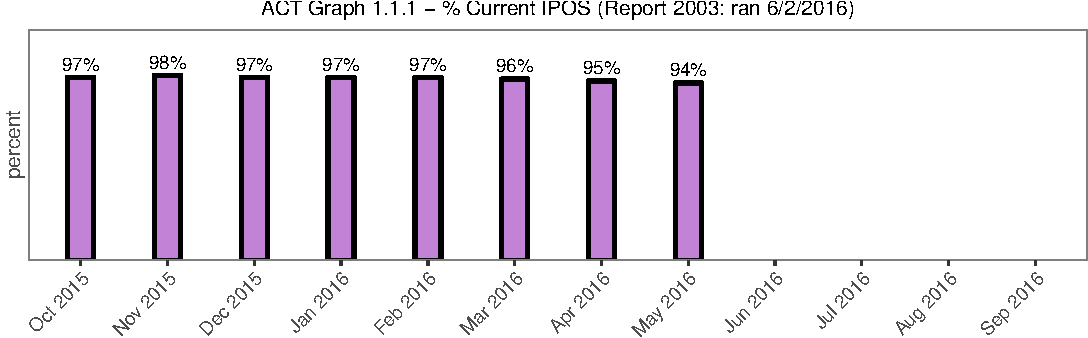
\includegraphics[width=\maxwidth]{figure/ACT_hist-1} 

\end{knitrout}

\begin{minipage}{\linewidth} { ACT: IPOS Table 1.1.1 \newline } % latex table generated in R 3.2.3 by xtable 1.8-0 package
% Tue Jan 05 22:52:49 2016
\scalebox{0.8}{
\begin{tabular}{p{0.10 \textwidth}|p{0.08 \textwidth}p{0.14 \textwidth}p{0.08 \textwidth}}
  \toprule
\textbf{month} & \textbf{current IPOS} & \textbf{blank/missing IPOS} & \textbf{expired IPOS} \\ 
  \midrule
Oct 2015 & 114 &   0 &   3 \\ 
  Nov 2015 & 116 &   0 &   2 \\ 
  Dec 2015 & 116 &   0 &   4 \\ 
   \bottomrule
\end{tabular}
}
 \par \bigskip \end{minipage}

\begin{minipage}{\linewidth} { ACT: IPOS Table 1.1.2 \newline } % latex table generated in R 3.2.3 by xtable 1.8-0 package
% Tue Jan 05 22:52:49 2016
\scalebox{0.8}{
\begin{tabular}{p{0.1\textwidth}|p{0.07\textwidth}p{0.07\textwidth}p{0.14 \textwidth}p{0.14\textwidth}p{0.15\textwidth}|p{0.08\textwidth}}
  \toprule
\textbf{month} & \textbf{Full IPOS} & \textbf{Interim IPOS} & \textbf{Interim IPOS Over 30 Days} & \textbf{Preliminary IPOS} & \textbf{Single Service IPOS} & \textbf{Grand Total} \\ 
  \midrule
Oct 2015 & 116 &   0 &   0 &   1 &   0 & 117 \\ 
  Nov 2015 & 117 &   1 &   0 &   0 &   0 & 118 \\ 
  Dec 2015 & 120 &   0 &   0 &   0 &   0 & 120 \\ 
   \bottomrule
\end{tabular}
}
 \par \bigskip \end{minipage}

\begin{minipage}{\linewidth} { ACT: IPOS Table 1.1.3 \newline } % latex table generated in R 3.2.3 by xtable 1.8-0 package
% Tue Jan 05 22:52:49 2016
\scalebox{0.8}{
\begin{tabular}{p{0.15\textwidth}|p{0.15\textwidth}p{0.25\textwidth}}
  \toprule
\textbf{supervisor} & \textbf{primary staff} & \textbf{expired/missing IPOS} \\ 
  \midrule
\textbf{Rahn, Nathan} &  & \hspace{2cm}\textbf{\textbf{2}} \\ 
   & Ing, Daniel & 2 \\ 
  \textbf{Schrader, Lisa} &  & \hspace{2cm}\textbf{\textbf{2}} \\ 
   \rowcolor[gray]{0.90} & Messina, Heather & 2 \\ 
   \bottomrule
\end{tabular}
}
 \par \bigskip \end{minipage}

\begin{absolutelynopagebreak}
\subsection{Unsigned/Draft Documents}
\begin{knitrout}
\definecolor{shadecolor}{rgb}{0.969, 0.969, 0.969}\color{fgcolor}
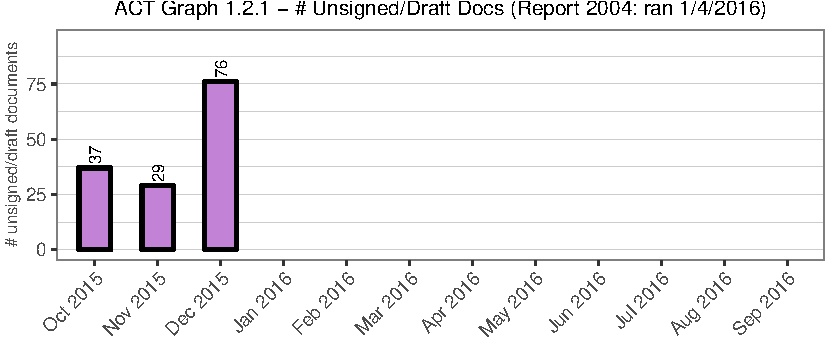
\includegraphics[width=\maxwidth]{figure/ACT_p_unsign-1} 

\end{knitrout}
\end{absolutelynopagebreak}

%' \begin{absolutelynopagebreak}
%' \subsection{Demographic Errors}
%' <<ACT_p_demo, fig.show="hold", message=FALSE, echo=FALSE, fig.height=2.25, fig.width=5.5>>=
%' p_demo[[1]]
%' @
%' \end{absolutelynopagebreak}

%' \begin{absolutelynopagebreak}
%' \subsection{Health Errors}
%' <<ACT_p_health, fig.show="hold", message=FALSE, echo=FALSE, fig.height=2.25, fig.width=5.5>>=
%' p_health[[1]]
%' @
%' \end{absolutelynopagebreak}

%' \begin{absolutelynopagebreak}
%' \subsection{Minimum Wage Errors}
%' <<ACT_p_wage, fig.show="hold", message=FALSE, echo=FALSE, fig.height=2.25, fig.width=5.5>>=
%' p_wage[[1]]
%' @
%' \end{absolutelynopagebreak}

%%%%%%%%% CHILDREN'S SERVICES %%%%%%%%%%%%%%%%%%%%%%%%%%%%%%%%
% \begin{absolutelynopagebreak}
\section{Children's Services}
\subsection{IPOS}
\begin{knitrout}
\definecolor{shadecolor}{rgb}{0.969, 0.969, 0.969}\color{fgcolor}
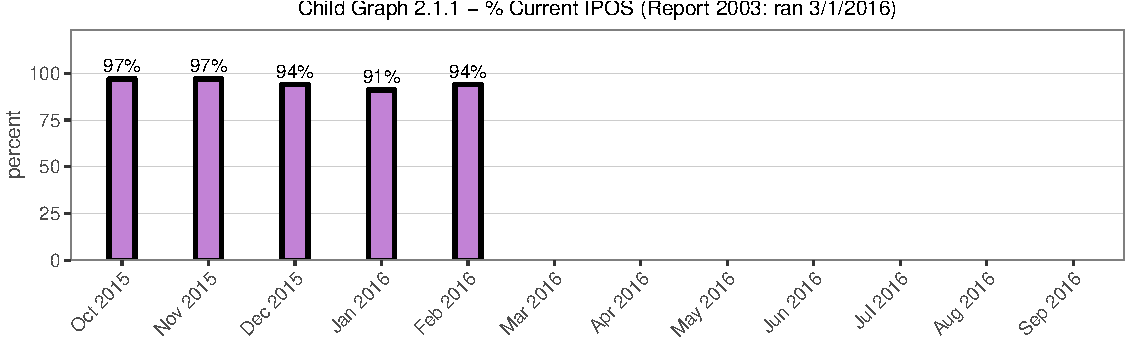
\includegraphics[width=\maxwidth]{figure/child_hist-1} 

\end{knitrout}
% \end{absolutelynopagebreak}

\begin{minipage}{\linewidth} { Children's Services: IPOS Table 2.1.1 \newline } % latex table generated in R 3.2.3 by xtable 1.8-0 package
% Tue Jan 05 22:52:50 2016
\scalebox{0.8}{
\begin{tabular}{p{0.10 \textwidth}|p{0.08 \textwidth}p{0.14 \textwidth}p{0.08 \textwidth}}
  \toprule
\textbf{month} & \textbf{current IPOS} & \textbf{blank/missing IPOS} & \textbf{expired IPOS} \\ 
  \midrule
Oct 2015 & 525 &   0 &  16 \\ 
  Nov 2015 & 527 &   0 &  16 \\ 
  Dec 2015 & 503 &   0 &  41 \\ 
   \bottomrule
\end{tabular}
}
 \par \bigskip \end{minipage}

\begin{minipage}{\linewidth} { Children's Services: IPOS Table 2.1.2 \newline } % latex table generated in R 3.2.3 by xtable 1.8-0 package
% Tue Jan 05 22:52:50 2016
\scalebox{0.8}{
\begin{tabular}{p{0.1\textwidth}|p{0.07\textwidth}p{0.07\textwidth}p{0.14\textwidth}p{0.14\textwidth}p{0.15\textwidth}|p{0.08\textwidth}}
  \toprule
\textbf{month} & \textbf{Full IPOS} & \textbf{Interim IPOS} & \textbf{Interim IPOS Over 30 Days} & \textbf{Preliminary IPOS} & \textbf{Single Service IPOS} & \textbf{Grand Total} \\ 
  \midrule
Oct 2015 & 508 &   1 &   0 &  32 &   0 & 541 \\ 
  Nov 2015 & 510 &   1 &   0 &  32 &   0 & 543 \\ 
  Dec 2015 & 508 &   1 &   0 &  35 &   0 & 544 \\ 
   \bottomrule
\end{tabular}
}
 \par \bigskip \end{minipage}

\begin{minipage}{\linewidth} { Children's Services: IPOS Table 2.1.3 \newline } % latex table generated in R 3.2.3 by xtable 1.8-0 package
% Tue Jan 05 22:52:50 2016
\scalebox{0.8}{
\begin{tabular}{p{0.18\textwidth}|p{0.20\textwidth}p{0.25\textwidth}}
  \toprule
\textbf{supervisor} & \textbf{primary staff} & \textbf{expired/missing IPOS} \\ 
  \midrule
\textbf{Brookens-Harvey, Barbara} &  & \hspace{2cm}\textbf{\textbf{7}} \\ 
   & Hill, Mikki & 2 \\ 
   & Love, Sarah & 2 \\ 
   \rowcolor[gray]{0.90} & Mathison, Shannon & 1 \\ 
   \rowcolor[gray]{0.90} & Womack, Nicole & 2 \\ 
   \rowcolor[gray]{0.90}\textbf{Hapeman, Christine} &  & \hspace{2cm}\textbf{\textbf{29}} \\ 
   & Angeski-Barron, Michelle & 1 \\ 
   & Burnett, Karen & 4 \\ 
   & Ferguson, Peter & 7 \\ 
   \rowcolor[gray]{0.90} & Fortune, Barbara & 11 \\ 
   \rowcolor[gray]{0.90} & Groth, Melissa & 1 \\ 
   \rowcolor[gray]{0.90} & Jennings, Margaret & 2 \\ 
   & Rivest, Christina & 2 \\ 
   & Sulfaro, Laura & 1 \\ 
  \textbf{LeVar, Sarah} &  & \hspace{2cm}\textbf{\textbf{8}} \\ 
   \rowcolor[gray]{0.90} & Bauer, Ann & 2 \\ 
   \rowcolor[gray]{0.90} & Hall, Philip & 2 \\ 
   \rowcolor[gray]{0.90} & Thurman, Judith & 4 \\ 
   \bottomrule
\end{tabular}
}
 \par \bigskip \end{minipage}

\begin{absolutelynopagebreak}
\subsection{Unsigned/Draft Documents}
\begin{knitrout}
\definecolor{shadecolor}{rgb}{0.969, 0.969, 0.969}\color{fgcolor}
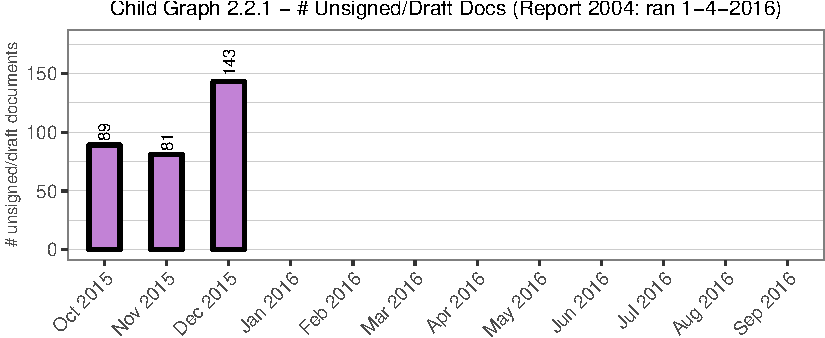
\includegraphics[width=\maxwidth]{figure/child_p_unsign-1} 

\end{knitrout}
\end{absolutelynopagebreak}

%' \begin{absolutelynopagebreak}
%' \subsection{Demographic Errors}
%' <<child_p_demo, fig.show="hold", message=FALSE, echo=FALSE, fig.height=2.25, fig.width=5.5>>=
%' p_demo[[2]]
%' @
%' \end{absolutelynopagebreak}

%' \begin{absolutelynopagebreak}
%' \subsection{Health Errors}
%' <<child_p_health, fig.show="hold", message=FALSE, echo=FALSE, fig.height=2.25, fig.width=5.5>>=
%' p_health[[2]]
%' @
%' \end{absolutelynopagebreak}

%' \begin{absolutelynopagebreak}
%' \subsection{Minimum Wage Errors}
%' <<child_p_wage, fig.show="hold", message=FALSE, echo=FALSE, fig.height=2.25, fig.width=5.5>>=
%' p_wage[[2]]
%' @
%' \end{absolutelynopagebreak}

%%%%%%%%%% Children's Services Home Based %%%%%%%%%%%%%%%%%%%
\pagebreak
\section{Children's Services Home Based}
\subsection{IPOS}
\begin{knitrout}
\definecolor{shadecolor}{rgb}{0.969, 0.969, 0.969}\color{fgcolor}
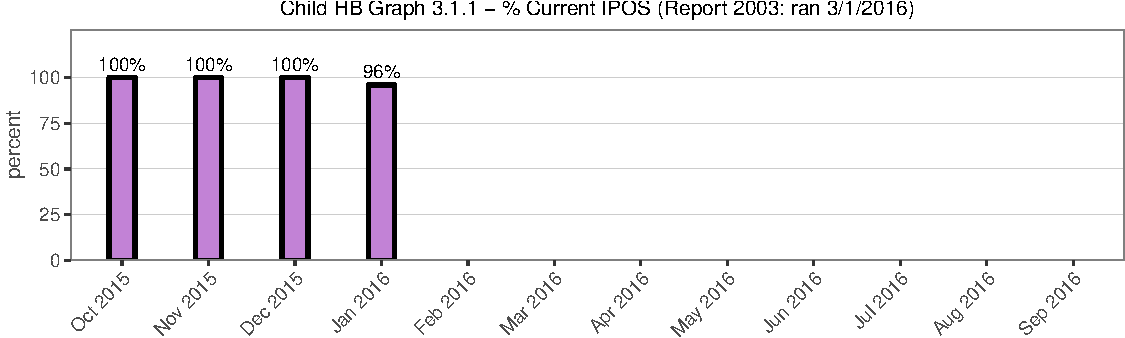
\includegraphics[width=\maxwidth]{figure/hb_hist-1} 

\end{knitrout}

\begin{minipage}{\linewidth} { Children's Services Home Based: IPOS Table 3.1.1 \newline } % latex table generated in R 3.2.3 by xtable 1.8-0 package
% Tue Jan 05 22:52:51 2016
\scalebox{0.8}{
\begin{tabular}{p{0.10 \textwidth}|p{0.08 \textwidth}p{0.14 \textwidth}p{0.08 \textwidth}}
  \toprule
\textbf{month} & \textbf{current IPOS} & \textbf{blank/missing IPOS} & \textbf{expired IPOS} \\ 
  \midrule
Oct 2015 &  27 &   0 &   0 \\ 
  Nov 2015 &  26 &   0 &   0 \\ 
  Dec 2015 &  22 &   0 &   1 \\ 
   \bottomrule
\end{tabular}
}
 \par \bigskip \end{minipage}

\begin{minipage}{\linewidth} { Children's Services Home Based: IPOS Table 3.1.2 \newline } % latex table generated in R 3.2.3 by xtable 1.8-0 package
% Tue Jan 05 22:52:51 2016
\scalebox{0.8}{
\begin{tabular}{p{0.1\textwidth}|p{0.07\textwidth}p{0.07\textwidth}p{0.14\textwidth}p{0.14\textwidth}p{0.15\textwidth}|p{0.08\textwidth}}
  \toprule
\textbf{month} & \textbf{Full IPOS} & \textbf{Interim IPOS} & \textbf{Interim IPOS Over 30 Days} & \textbf{Preliminary IPOS} & \textbf{Single Service IPOS} & \textbf{Grand Total} \\ 
  \midrule
Oct 2015 &  27 &   0 &   0 &   0 &   0 &  27 \\ 
  Nov 2015 &  26 &   0 &   0 &   0 &   0 &  26 \\ 
  Dec 2015 &  23 &   0 &   0 &   0 &   0 &  23 \\ 
   \bottomrule
\end{tabular}
}
 \par \bigskip \end{minipage}

\begin{minipage}{\linewidth} { Children's Services Home Based: IPOS Table 3.1.3 \newline } % latex table generated in R 3.2.3 by xtable 1.8-0 package
% Tue Jan 05 22:52:51 2016
\scalebox{0.8}{
\begin{tabular}{p{0.15\textwidth}|p{0.15\textwidth}p{0.25\textwidth}}
  \toprule
\textbf{supervisor} & \textbf{primary staff} & \textbf{expired/missing IPOS} \\ 
  \midrule
\textbf{Brookens-Harvey, Barbara} &  & \hspace{2cm}\textbf{\textbf{1}} \\ 
   & Womack, Nicole & 1 \\ 
   \bottomrule
\end{tabular}
}
 \par \bigskip \end{minipage}

\begin{absolutelynopagebreak}
\subsection{Unsigned/Draft Documents}
\begin{knitrout}
\definecolor{shadecolor}{rgb}{0.969, 0.969, 0.969}\color{fgcolor}
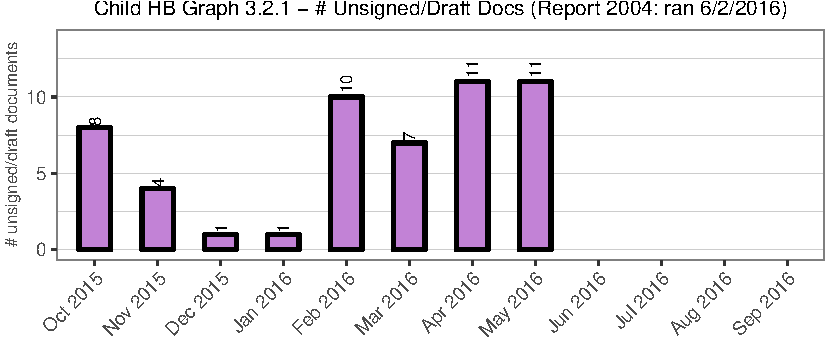
\includegraphics[width=\maxwidth]{figure/hb_p_unsign-1} 

\end{knitrout}
\end{absolutelynopagebreak}

%' \begin{absolutelynopagebreak}
%' \subsection{Demographic Errors}
%' <<hb_p_demo, fig.show="hold", message=FALSE, echo=FALSE, fig.height=2.25, fig.width=5.5>>=
%' p_demo[[3]]
%' @
%' \end{absolutelynopagebreak}

%' \begin{absolutelynopagebreak}
%' \subsection{Health Errors}
%' <<hb_p_health, fig.show="hold", message=FALSE, echo=FALSE, fig.height=2.25, fig.width=5.5>>=
%' p_health[[3]]
%' @
%' \end{absolutelynopagebreak}

%%%%%%%%%% DD Adult %%%%%%%%%%%%%%%%%%%%%%
\pagebreak
\section{DD Adult}
\subsection{IPOS}
\begin{knitrout}
\definecolor{shadecolor}{rgb}{0.969, 0.969, 0.969}\color{fgcolor}
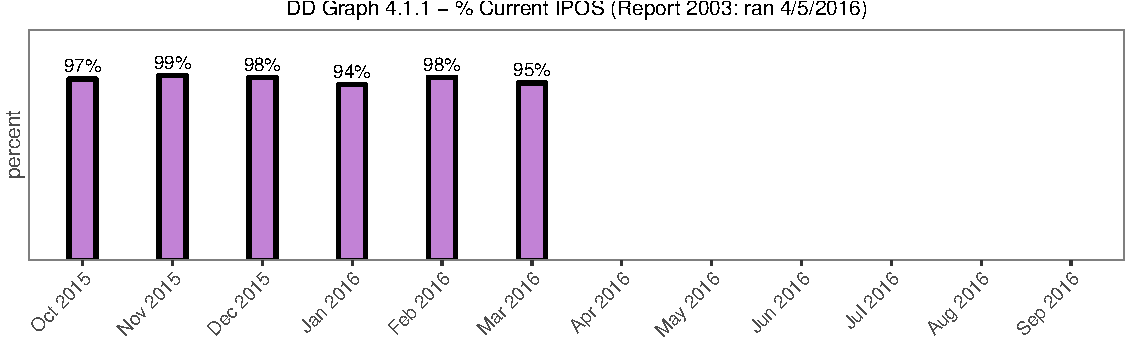
\includegraphics[width=\maxwidth]{figure/dd_hist-1} 

\end{knitrout}

\begin{minipage}{\linewidth} { DD Adult: IPOS Table 4.1.1 \newline } % latex table generated in R 3.2.3 by xtable 1.8-0 package
% Tue Jan 05 22:52:52 2016
\scalebox{0.8}{
\begin{tabular}{p{0.10 \textwidth}|p{0.08 \textwidth}p{0.14 \textwidth}p{0.08 \textwidth}}
  \toprule
\textbf{month} & \textbf{current IPOS} & \textbf{blank/missing IPOS} & \textbf{expired IPOS} \\ 
  \midrule
Oct 2015 & 892 &   0 &  31 \\ 
  Nov 2015 & 921 &   0 &  10 \\ 
  Dec 2015 & 899 &   0 &  29 \\ 
   \bottomrule
\end{tabular}
}
 \par \bigskip \end{minipage}

\begin{minipage}{\linewidth} { DD Adult: IPOS Table 4.1.2 \newline } % latex table generated in R 3.2.3 by xtable 1.8-0 package
% Tue Jan 05 22:52:53 2016
\scalebox{0.8}{
\begin{tabular}{p{0.1\textwidth}|p{0.07\textwidth}p{0.07\textwidth}p{0.14\textwidth}p{0.14\textwidth}p{0.15\textwidth}|p{0.08\textwidth}}
  \toprule
\textbf{month} & \textbf{Full IPOS} & \textbf{Interim IPOS} & \textbf{Interim IPOS Over 30 Days} & \textbf{Preliminary IPOS} & \textbf{Single Service IPOS} & \textbf{Grand Total} \\ 
  \midrule
Oct 2015 & 896 &  10 &   1 &   6 &  11 & 923 \\ 
  Nov 2015 & 901 &  10 &   1 &   9 &  11 & 931 \\ 
  Dec 2015 & 902 &   9 &   3 &   6 &  11 & 928 \\ 
   \bottomrule
\end{tabular}
}
 \par \bigskip \end{minipage}

\begin{minipage}{\linewidth} { DD Adult: IPOS Table 4.1.3 \newline } % latex table generated in R 3.2.3 by xtable 1.8-0 package
% Tue Jan 05 22:52:53 2016
\scalebox{0.8}{
\begin{tabular}{p{0.15\textwidth}|p{0.25\textwidth}p{0.25\textwidth}}
  \toprule
\textbf{supervisor} & \textbf{primary staff} & \textbf{expired/missing IPOS} \\ 
  \midrule
\textbf{Diephuis, Krista} &  & \hspace{2cm}\textbf{\textbf{2}} \\ 
   & Greenleaf, Daryl & 1 \\ 
   & Wells, Tracy & 1 \\ 
   \rowcolor[gray]{0.90}\textbf{Dronamraju, Rani} &  & \hspace{2cm}\textbf{\textbf{2}} \\ 
   \rowcolor[gray]{0.90} & Lawson Chukwudi, Patricia & 1 \\ 
   \rowcolor[gray]{0.90} & McClain, Ashley & 1 \\ 
  \textbf{Mohring, Kathleen} &  & \hspace{2cm}\textbf{\textbf{15}} \\ 
   & Karm, Thomas & 1 \\ 
   & Mackenzie, Deborah & 8 \\ 
   \rowcolor[gray]{0.90} & Moore, Carmen & 5 \\ 
   \rowcolor[gray]{0.90} & Terry, Yvette & 1 \\ 
   \rowcolor[gray]{0.90}\textbf{Wells, Tracy} &  & \hspace{2cm}\textbf{\textbf{10}} \\ 
   & Fillman-Hatcher, Carolyn & 5 \\ 
   & Hoover, Danielle & 1 \\ 
   & Jacobs, Kevin & 1 \\ 
   \rowcolor[gray]{0.90} & Petty, Cheryl & 2 \\ 
   \rowcolor[gray]{0.90} & Schramm, Joshua & 1 \\ 
   \bottomrule
\end{tabular}
}
 \par \bigskip \end{minipage}

\begin{absolutelynopagebreak}
\subsection{Unsigned/Draft Documents}
\begin{knitrout}
\definecolor{shadecolor}{rgb}{0.969, 0.969, 0.969}\color{fgcolor}
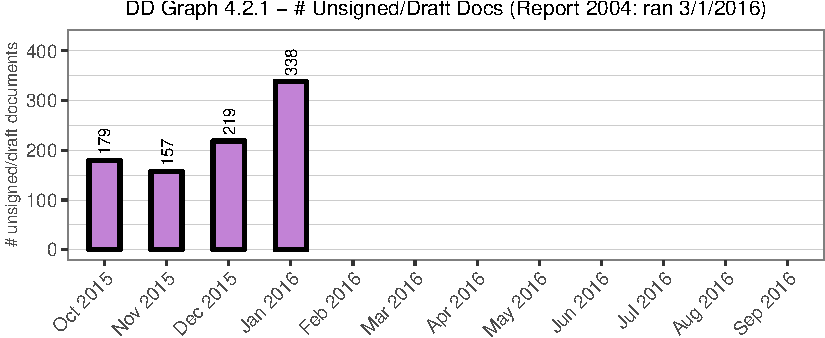
\includegraphics[width=\maxwidth]{figure/dd_p_unsign-1} 

\end{knitrout}
\end{absolutelynopagebreak}

%' \begin{absolutelynopagebreak}
%' \subsection{Demographic Errors}
%' <<dd_p_demo, fig.show="hold", message=FALSE, echo=FALSE, fig.height=2.25, fig.width=5.5>>=
%' p_demo[[4]]
%' @
%' \end{absolutelynopagebreak}

%' \begin{absolutelynopagebreak}
%' \subsection{Health Errors}
%' <<dd_p_health, fig.show="hold", message=FALSE, echo=FALSE, fig.height=2.25, fig.width=5.5>>=
%' p_health[[4]]
%' @
%' \end{absolutelynopagebreak}

%' % \begin{absolutelynopagebreak}
%' \subsection{Minimum Wage Errors}
%' <<dd_p_wage, fig.show="hold", message=FALSE, echo=FALSE, fig.height=2.25, fig.width=5.5>>=
%' p_wage[[4]]
%' @
%' % \end{absolutelynopagebreak}

%%%%%%%%%% MI Adult %%%%%%%%%%%%%%%%%%%%%
% \begin{absolutelynopagebreak}
\section{MI Adult}
\subsection{IPOS}
\begin{knitrout}
\definecolor{shadecolor}{rgb}{0.969, 0.969, 0.969}\color{fgcolor}
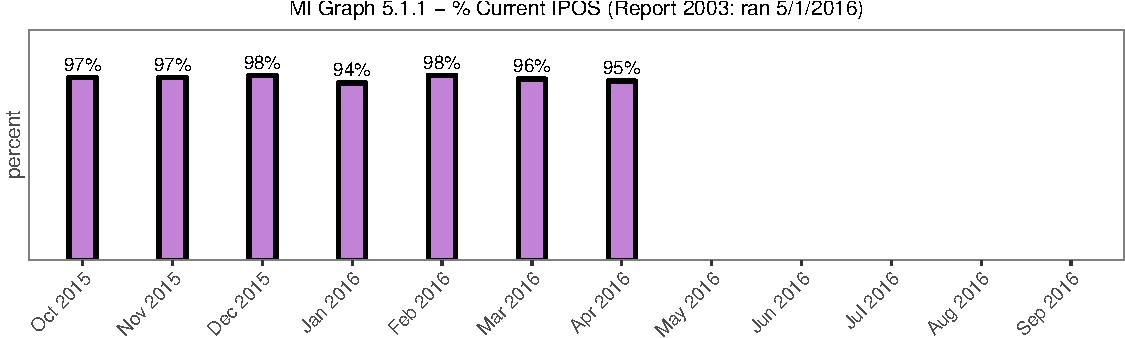
\includegraphics[width=\maxwidth]{figure/mi_hist-1} 

\end{knitrout}
% \end{absolutelynopagebreak}

\begin{minipage}{\linewidth} { MI Adult: IPOS Table 5.1.1 \newline } % latex table generated in R 3.2.3 by xtable 1.8-0 package
% Tue Jan 05 22:52:53 2016
\scalebox{0.8}{
\begin{tabular}{p{0.10 \textwidth}|p{0.08 \textwidth}p{0.14 \textwidth}p{0.08 \textwidth}}
  \toprule
\textbf{month} & \textbf{current IPOS} & \textbf{blank/missing IPOS} & \textbf{expired IPOS} \\ 
  \midrule
Oct 2015 & 1750 &   0 &  59 \\ 
  Nov 2015 & 1744 &   0 &  50 \\ 
  Dec 2015 & 1721 &   0 &  68 \\ 
   \bottomrule
\end{tabular}
}
 \par \bigskip \end{minipage}

\begin{minipage}{\linewidth} { MI Adult: IPOS Table 5.1.2 \newline } % latex table generated in R 3.2.3 by xtable 1.8-0 package
% Tue Jan 05 22:52:53 2016
\scalebox{0.8}{
\begin{tabular}{p{0.1\textwidth}|p{0.07\textwidth}p{0.07\textwidth}p{0.14\textwidth}p{0.14\textwidth}p{0.15\textwidth}|p{0.08\textwidth}}
  \toprule
\textbf{month} & \textbf{Full IPOS} & \textbf{Interim IPOS} & \textbf{Interim IPOS Over 30 Days} & \textbf{Preliminary IPOS} & \textbf{Single Service IPOS} & \textbf{Grand Total} \\ 
  \midrule
Oct 2015 & 1756 &   2 &   1 &  48 &   3 & 1809 \\ 
  Nov 2015 & 1740 &   6 &   2 &  45 &   3 & 1794 \\ 
  Dec 2015 & 1731 &  10 &   3 &  45 &   3 & 1789 \\ 
   \bottomrule
\end{tabular}
}
 \par \bigskip \end{minipage}

% latex table generated in R 3.2.3 by xtable 1.8-0 package
% Tue Jan 05 22:52:53 2016
\begin{longtable} { >{\raggedright}p{0.14\textwidth}|p{0.30\textwidth}p{0.25\textwidth}}
  \multicolumn{3}{l}{{MI Adult: IPOS Table 5.1.3}}\ \label{}\\  \toprule  \textbf{supervisor}  & \textbf{primary staff} & \textbf{expired/missing IPOS} \\\midrule  \endfirsthead  \multicolumn{3}{c}{{MI Adult: IPOS Table 5.1.3 -- continued from previous page}}\\  \toprule  \textbf{supervisor} & \textbf{primary staff}& \textbf{expired/missing IPOS} \\\midrule  \endhead  \midrule  \multicolumn{3}{r}{{Continued on next page}}\\  \bottomrule \endfoot  \bottomrule \endlastfoot  \textbf{Edwards, Sheri} &  & \hspace{2cm}\textbf{\textbf{37}} \\ 
   & Allen, Katekia & 6 \\ 
   & Beckley, Jeff & 2 \\ 
   \rowcolor[gray]{0.90} & Donald, Angela & 2 \\ 
   \rowcolor[gray]{0.90} & Johnson, Tamika & 7 \\ 
   \rowcolor[gray]{0.90} & McLemore, Sherry & 1 \\ 
   & Melody, Alex & 1 \\ 
   & O'Donnell, Alexandra & 1 \\ 
   & Thomas, Kristian & 4 \\ 
   \rowcolor[gray]{0.90} & Tisdale, Tina & 1 \\ 
   \rowcolor[gray]{0.90} & Toole, Keisha & 4 \\ 
   \rowcolor[gray]{0.90} & Wright, Christine & 8 \\ 
  \textbf{Gentz, Judith} &  & \hspace{2cm}\textbf{\textbf{1}} \\ 
   & Meadows, Cassandra & 1 \\ 
  \textbf{Hoener, Katie} &  & \hspace{2cm}\textbf{\textbf{2}} \\ 
   \rowcolor[gray]{0.90} & Lampe, Mary & 2 \\ 
   \rowcolor[gray]{0.90}\textbf{Schrader, Lisa} &  & \hspace{2cm}\textbf{\textbf{10}} \\ 
   \rowcolor[gray]{0.90} & Brouwer, Patricia & 1 \\ 
   & Davis, Shauntai & 6 \\ 
   & Miron, Jason & 1 \\ 
   & Reid, Courtney & 2 \\ 
   \rowcolor[gray]{0.90}\textbf{Sheng, Mei-fu} &  & \hspace{2cm}\textbf{\textbf{2}} \\ 
   \rowcolor[gray]{0.90} & Stacy, John & 2 \\ 
   \rowcolor[gray]{0.90}\textbf{Shovels, John} &  & \hspace{2cm}\textbf{\textbf{2}} \\ 
   & Edwards, Sheri & 2 \\ 
  \textbf{Stacy, John} &  & \hspace{2cm}\textbf{\textbf{10}} \\ 
   & Bennett, Sarah & 1 \\ 
   \rowcolor[gray]{0.90} & Blach, Aura & 5 \\ 
   \rowcolor[gray]{0.90} & Koch, Lynn & 1 \\ 
   \rowcolor[gray]{0.90} & Sims, Elaina & 3 \\ 
  \textbf{Thacker, Barbara} &  & \hspace{2cm}\textbf{\textbf{5}} \\ 
   & Perry, Meredith & 5 \\ 
  none/missing &  & 1 \\ 
   \rowcolor[gray]{0.90}\textbf{NA} &  & \hspace{2cm}\textbf{\textbf{1}} \\ 
   \end{longtable}


\begin{absolutelynopagebreak}
\subsection{Unsigned/Draft Documents}
\begin{knitrout}
\definecolor{shadecolor}{rgb}{0.969, 0.969, 0.969}\color{fgcolor}
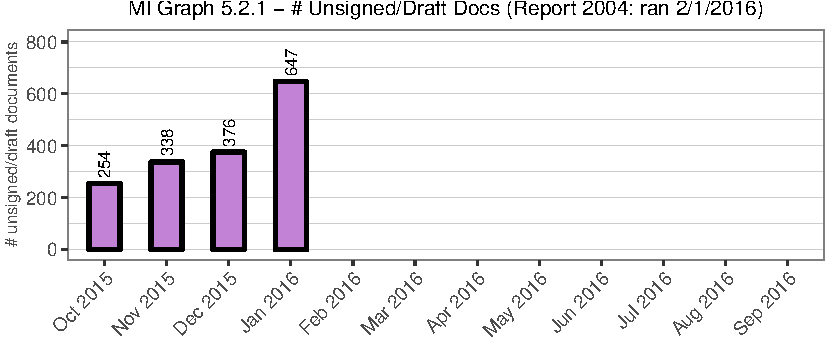
\includegraphics[width=\maxwidth]{figure/mi_p_unsign-1} 

\end{knitrout}
\end{absolutelynopagebreak}

%' \begin{absolutelynopagebreak}
%' \subsection{Demographic Errors}
%' <<mi_p_demo, fig.show="hold", message=FALSE, echo=FALSE, fig.height=2.25, fig.width=5.5>>=
%' p_demo[[5]]
%' @
%' \end{absolutelynopagebreak}

%' \subsection{Health Errors}
%' <<mi_p_health, fig.show="hold", message=FALSE, echo=FALSE, fig.height=2.25, fig.width=5.5>>=
%' p_health[[5]]
%' @

%' \begin{absolutelynopagebreak}
%' \subsection{Minimum Wage Errors}
%' <<mi_p_wage, fig.show="hold", message=FALSE, echo=FALSE, fig.height=2.25, fig.width=5.5>>=
%' p_wage[[5]]
%' @
%' \end{absolutelynopagebreak}

\pagebreak
\section{Unsigned and Draft Documents}
Unsigned/Draft Documents by Supervisor/Enterer - Report 2004: ran 1-4-2016 \newline
\small{
% latex table generated in R 3.2.3 by xtable 1.8-0 package
% Tue Jan 05 22:52:54 2016
\begin{longtable} { >{\raggedright}p{0.25\textwidth}|p{0.27\textwidth}p{0.22\textwidth}}
  \multicolumn{3}{l}{{Table 6.1}}\ \label{}\\  \toprule  \textbf{supervisor}  & \textbf{author} & \textbf{unsigned/draft docs} \\\midrule  \endfirsthead  \multicolumn{3}{c}{{Table 6.1 -- continued from previous page}}\\  \toprule  \textbf{supervisor} & \textbf{author}& \textbf{unsigned/draft docs} \\\midrule  \endhead  \midrule  \multicolumn{3}{r}{{Continued on next page}}\\  \bottomrule \endfoot  \bottomrule \endlastfoot  \textbf{Bellus, Kelly} &  & \hspace{2cm}\textbf{3} \\ 
   & Ricketts, Kathleen & 1 \\ 
   & Swisher, Stephanie & 2 \\ 
   \rowcolor[gray]{0.90}\textbf{Brookens-Harvey, Barbara} &  & \hspace{2cm}\textbf{16} \\ 
   \rowcolor[gray]{0.90} & Burton, Alexia & 1 \\ 
   \rowcolor[gray]{0.90} & Ellis, Shannon & 2 \\ 
   & Hill, Mikki & 1 \\ 
   & Love, Sarah & 1 \\ 
   & McClure, Eric & 9 \\ 
   \rowcolor[gray]{0.90} & Womack, Nicole & 2 \\ 
   \rowcolor[gray]{0.90}\textbf{Chisholm, Debra} &  & \hspace{2cm}\textbf{6} \\ 
   \rowcolor[gray]{0.90} & Marshall, Deitra & 4 \\ 
   & Philpot, Mary & 2 \\ 
  \textbf{Cortes, Patricia} &  & \hspace{2cm}\textbf{2} \\ 
   & Florence, Timothy & 2 \\ 
   \rowcolor[gray]{0.90}\textbf{Diephuis, Krista} &  & \hspace{2cm}\textbf{3} \\ 
   \rowcolor[gray]{0.90} & Gilkey, Jenoah & 3 \\ 
   \rowcolor[gray]{0.90}\textbf{Dronamraju, Rani} &  & \hspace{2cm}\textbf{36} \\ 
   & Bryant, Biancia & 4 \\ 
   & Erickson, Sara & 2 \\ 
   & Ernst, Jessica & 1 \\ 
   \rowcolor[gray]{0.90} & Fenner, Caryette & 6 \\ 
   \rowcolor[gray]{0.90} & Lawson Chukwudi, Patricia & 13 \\ 
   \rowcolor[gray]{0.90} & McClain, Ashley & 1 \\ 
   & Nurmi, Bill & 3 \\ 
   & Quine, Daniel & 2 \\ 
   & Trinka, Lisa & 1 \\ 
   \rowcolor[gray]{0.90} & Yu, Lucia & 3 \\ 
   \rowcolor[gray]{0.90}\textbf{Edwards, Sheri} &  & \hspace{2cm}\textbf{117} \\ 
   \rowcolor[gray]{0.90} & Allen, Katekia & 17 \\ 
   & Aseltyne, Sarah & 3 \\ 
   & Atwell, Andrea & 6 \\ 
   & Bajema, Stacey & 6 \\ 
   \rowcolor[gray]{0.90} & Beckley, Jeff & 4 \\ 
   \rowcolor[gray]{0.90} & Beland, Darren & 12 \\ 
   \rowcolor[gray]{0.90} & Blaze, Renee & 4 \\ 
   & Dempsey, Kelsey & 3 \\ 
   & Johnson, Tamika & 1 \\ 
   & Jordan, Shad & 2 \\ 
   \rowcolor[gray]{0.90} & McLemore, Sherry & 13 \\ 
   \rowcolor[gray]{0.90} & Melody, Alex & 2 \\ 
   \rowcolor[gray]{0.90} & O'Donnell, Alexandra & 6 \\ 
   & Svensson, Kathy & 5 \\ 
   & Thomas, Kristian & 7 \\ 
   & Tisdale, Tina & 7 \\ 
   \rowcolor[gray]{0.90} & Toole, Keisha & 12 \\ 
   \rowcolor[gray]{0.90} & Wright, Christine & 7 \\ 
   \rowcolor[gray]{0.90}\textbf{Florence, Timothy} &  & \hspace{2cm}\textbf{390} \\ 
   & Bright, Jessica & 6 \\ 
   & Demehri, Angela & 3 \\ 
   & Edwards, Lauren & 1 \\ 
   \rowcolor[gray]{0.90} & Gargan, Michele & 2 \\ 
   \rowcolor[gray]{0.90} & Gentz, Judith & 5 \\ 
   \rowcolor[gray]{0.90} & Hashimoto, Martha & 9 \\ 
   & Healy III, Daniel & 43 \\ 
   & Husby, Leah & 28 \\ 
   & Mayman, Daniel & 6 \\ 
   \rowcolor[gray]{0.90} & Mobilio, Andrea & 74 \\ 
   \rowcolor[gray]{0.90} & Shauger, Michelle & 10 \\ 
   \rowcolor[gray]{0.90} & Stetz, Sharon & 59 \\ 
   & Washington, W. Craig & 135 \\ 
   & Young, Martha & 9 \\ 
  \textbf{Gentz, Lisa} &  & \hspace{2cm}\textbf{1} \\ 
   \rowcolor[gray]{0.90} & Leadford, William & 1 \\ 
   \rowcolor[gray]{0.90}\textbf{Hagaman, Brandie} &  & \hspace{2cm}\textbf{16} \\ 
   \rowcolor[gray]{0.90} & Fellabaum, Kathleen & 2 \\ 
   & Hershberger, Merton & 4 \\ 
   & Lewis, Destiny & 4 \\ 
   & Rama, Linda & 5 \\ 
   \rowcolor[gray]{0.90} & VanHoeck, Marie & 1 \\ 
   \rowcolor[gray]{0.90}\textbf{Hapeman, Christine} &  & \hspace{2cm}\textbf{28} \\ 
   \rowcolor[gray]{0.90} & Brookens-Harvey, Barbara & 2 \\ 
   & Burnett, Karen & 6 \\ 
   & Ferguson, Peter & 1 \\ 
   & Fortune, Barbara & 12 \\ 
   \rowcolor[gray]{0.90} & Grace, Carmen & 1 \\ 
   \rowcolor[gray]{0.90} & Groth, Melissa & 2 \\ 
   \rowcolor[gray]{0.90} & Jennings, Margaret & 2 \\ 
   & Rivest, Christina & 1 \\ 
   & Sulfaro, Laura & 1 \\ 
  \textbf{Hoener, Katie} &  & \hspace{2cm}\textbf{8} \\ 
   \rowcolor[gray]{0.90} & Lampe, Mary & 2 \\ 
   \rowcolor[gray]{0.90} & MacCormack, Catherine & 4 \\ 
   \rowcolor[gray]{0.90} & Twigg, Scott & 1 \\ 
   & Xia, Jingjing & 1 \\ 
  \textbf{Knapp, Timothy} &  & \hspace{2cm}\textbf{5} \\ 
   & Ghedotte, Janette & 3 \\ 
   \rowcolor[gray]{0.90} & Okonowski, Erich & 1 \\ 
   \rowcolor[gray]{0.90} & Pearson, Thomas & 1 \\ 
   \rowcolor[gray]{0.90}\textbf{Kroll, Phillip} &  & \hspace{2cm}\textbf{2} \\ 
   & Wright, Paul & 2 \\ 
  \textbf{LeVar, Sarah} &  & \hspace{2cm}\textbf{35} \\ 
   & Depp, John & 7 \\ 
   \rowcolor[gray]{0.90} & Hall, Philip & 2 \\ 
   \rowcolor[gray]{0.90} & Iekel-Johnson, Susan & 1 \\ 
   \rowcolor[gray]{0.90} & Leadford, Elizabeth & 9 \\ 
   & Perez, Irene & 4 \\ 
   & Starr, Catherine & 11 \\ 
   & Thurman, Judith & 1 \\ 
   \rowcolor[gray]{0.90}\textbf{Leadford, William} &  & \hspace{2cm}\textbf{26} \\ 
   \rowcolor[gray]{0.90} & Badri, Soumaya & 1 \\ 
   \rowcolor[gray]{0.90} & Benton-Brown, Miayana & 18 \\ 
   & Burchard, Angela & 1 \\ 
   & Hyde, Hannah & 2 \\ 
   & Karol, Tiffany & 1 \\ 
   \rowcolor[gray]{0.90} & Lloyd, Sylvia & 3 \\ 
   \rowcolor[gray]{0.90}\textbf{Mohring, Kathleen} &  & \hspace{2cm}\textbf{70} \\ 
   \rowcolor[gray]{0.90} & Allen, Brandy & 3 \\ 
   & Axberg, Stephanie & 15 \\ 
   & Ferriter, Michael & 10 \\ 
   & Karm, Thomas & 2 \\ 
   \rowcolor[gray]{0.90} & Lovelace, Julie & 20 \\ 
   \rowcolor[gray]{0.90} & Mackenzie, Deborah & 6 \\ 
   \rowcolor[gray]{0.90} & McMillon, Tracy & 5 \\ 
   & Moore, Carmen & 5 \\ 
   & Terry, Yvette & 4 \\ 
  \textbf{O'brien, Colleen} &  & \hspace{2cm}\textbf{8} \\ 
   \rowcolor[gray]{0.90} & Battle, Lanita & 1 \\ 
   \rowcolor[gray]{0.90} & Farrow, Marlene & 7 \\ 
   \rowcolor[gray]{0.90}\textbf{Owen, Debra} &  & \hspace{2cm}\textbf{45} \\ 
   & Cross, Ericka & 7 \\ 
   & Hartman, LaShanda & 3 \\ 
   & Hartmann, Robert & 7 \\ 
   \rowcolor[gray]{0.90} & Jasmund, Faith & 13 \\ 
   \rowcolor[gray]{0.90} & Mack, Kristian & 7 \\ 
   \rowcolor[gray]{0.90} & Spink, Nancy & 6 \\ 
   & Taylor, Stephen & 2 \\ 
  \textbf{Paxton, Britt} &  & \hspace{2cm}\textbf{62} \\ 
   & Lappo, Elizabeth & 28 \\ 
   \rowcolor[gray]{0.90} & Pilarski, Katherine & 3 \\ 
   \rowcolor[gray]{0.90} & Sommerville, Tomekia & 1 \\ 
   \rowcolor[gray]{0.90} & Thompson, Susan & 4 \\ 
   & Willis, Keisha & 26 \\ 
  \textbf{Rahn, Nathan} &  & \hspace{2cm}\textbf{49} \\ 
   & Behm, Emily & 1 \\ 
   \rowcolor[gray]{0.90} & Burpee, Elena & 5 \\ 
   \rowcolor[gray]{0.90} & Goode, Casey & 2 \\ 
   \rowcolor[gray]{0.90} & Halliday, Jessica & 4 \\ 
   & Hoogerhyde, Jill & 9 \\ 
   & Ing, Daniel & 6 \\ 
   & Scott, Vivian & 1 \\ 
   \rowcolor[gray]{0.90} & Srivastava, Sabreen & 15 \\ 
   \rowcolor[gray]{0.90} & Vanderlooven, Douglas & 6 \\ 
   \rowcolor[gray]{0.90}\textbf{Sattler, Lydia} &  & \hspace{2cm}\textbf{43} \\ 
   & Adkins, Douglas & 5 \\ 
   & Allen, Michelle & 8 \\ 
   & Beuckelaere, Jacqueline & 8 \\ 
   \rowcolor[gray]{0.90} & Cloud, Alda & 10 \\ 
   \rowcolor[gray]{0.90} & Patterson, Frederick & 3 \\ 
   \rowcolor[gray]{0.90} & Shadbolt, Gail & 9 \\ 
  \textbf{Schrader, Lisa} &  & \hspace{2cm}\textbf{66} \\ 
   & Brouwer, Patricia & 5 \\ 
   & Davis, Shauntai & 16 \\ 
   \rowcolor[gray]{0.90} & Halstead, Yarrow & 3 \\ 
   \rowcolor[gray]{0.90} & Messina, Heather & 10 \\ 
   \rowcolor[gray]{0.90} & Millar, Thana & 1 \\ 
   & Miron, Jason & 5 \\ 
   & Mitchell, Holly & 15 \\ 
   & Ray, Pamela & 1 \\ 
   \rowcolor[gray]{0.90} & Reid, Courtney & 6 \\ 
   \rowcolor[gray]{0.90} & Rossman, Mary & 4 \\ 
   \rowcolor[gray]{0.90}\textbf{Sheng, Mei-fu} &  & \hspace{2cm}\textbf{1} \\ 
   & Stacy, John & 1 \\ 
  \textbf{Shovels, John} &  & \hspace{2cm}\textbf{30} \\ 
   & Edwards, Sheri & 2 \\ 
   \rowcolor[gray]{0.90} & Hoener, Katie & 1 \\ 
   \rowcolor[gray]{0.90} & Rahn, Nathan & 27 \\ 
   \rowcolor[gray]{0.90}\textbf{Stacy, John} &  & \hspace{2cm}\textbf{48} \\ 
   & Bennett, Sarah & 1 \\ 
   & Jabzanka, Thaddeus & 6 \\ 
   & Lewis, Andrew & 5 \\ 
   \rowcolor[gray]{0.90} & Michalowski, Bryan & 1 \\ 
   \rowcolor[gray]{0.90} & Noe, Tori & 1 \\ 
   \rowcolor[gray]{0.90} & Reina, Aaron & 1 \\ 
   & Ruggeberg (Wolters), Lisa & 2 \\ 
   & Sims, Elaina & 7 \\ 
   & Wakely, Ann & 4 \\ 
   \rowcolor[gray]{0.90} & Wilson, Terrance & 20 \\ 
   \rowcolor[gray]{0.90}\textbf{Stearns, Stephanie} &  & \hspace{2cm}\textbf{14} \\ 
   \rowcolor[gray]{0.90} & Pickard, Steven & 12 \\ 
   & Shaffer (Kniceley), Ashley & 2 \\ 
  \textbf{Thacker, Barbara} &  & \hspace{2cm}\textbf{4} \\ 
   & Perry, Meredith & 4 \\ 
   \rowcolor[gray]{0.90}\textbf{Wells, Tracy} &  & \hspace{2cm}\textbf{25} \\ 
   \rowcolor[gray]{0.90} & Dooley, Mary & 6 \\ 
   \rowcolor[gray]{0.90} & Fillman-Hatcher, Carolyn & 1 \\ 
   & Jacobs, Kevin & 1 \\ 
   & Jacobs, Sarah & 1 \\ 
   & Petty, Cheryl & 1 \\ 
   \rowcolor[gray]{0.90} & Pickrel, April & 2 \\ 
   \rowcolor[gray]{0.90} & Schramm, Joshua & 1 \\ 
   \rowcolor[gray]{0.90} & Traverse, Laura & 3 \\ 
   & Umholtz, Elaine & 9 \\ 
  \textbf{Grand total} &  & \textbf{1159} \\ 
   \end{longtable}

}

\pagebreak

\section{Caseload and Not Seen 30/60/90/180 days}
Caseload and Not Seen 30/60/90/180 days (Report 2044: ran 1-4-2016)(No services at all) \newline
\small{
% latex table generated in R 3.2.3 by xtable 1.8-0 package
% Tue Jan 05 22:52:54 2016
\begin{longtable} { >{\raggedright}p{0.05\textwidth}p{0.22\textwidth}p{0.05\textwidth}p{0.09\textwidth}p{0.09\textwidth}p{0.09\textwidth}p{0.09\textwidth}p{0.09\textwidth}}
  \multicolumn{8}{l}{{Table 7.1}}\ \label{}\\  \toprule  \textbf{team}  & \textbf{primary staff} & \textbf{case load} & \textbf{level} & \textbf{not seen in 30 days} & \textbf{not seen in 60 days} & \textbf{not seen in 90 days} & \textbf{not seen in 180 days} \\\midrule  \endfirsthead  \multicolumn{8}{c}{{Table 7.1 -- continued from previous page}}\\  \toprule  \textbf{team} & \textbf{primary staff}& \textbf{case load}& \textbf{level}& \textbf{not seen in 30 days}& \textbf{not seen in 60 days}& \textbf{not seen in 90 days}& \textbf{not seen in 180 days} \\\midrule  \endhead  \midrule  \multicolumn{8}{r}{{Continued on next page}}\\  \bottomrule \endfoot  \bottomrule \endlastfoot  \textbf{ACT Team} &  & \textbf{120} & - & \textbf{13} & \textbf{7} & \textbf{6} & \textbf{2} \\ 
   & Halliday, Jessica & 11 & 4 & 2 & 1 & 1 & 0 \\ 
   & Ing, Daniel & 14 & 4 & 3 & 3 & 3 & 1 \\ 
   \rowcolor[gray]{0.90} & Jabzanka, Thaddeus & 14 & 4 & 1 & 1 & 1 & 0 \\ 
   \rowcolor[gray]{0.90} & Messina, Heather & 15 & 4 & 0 & 0 & 0 & 0 \\ 
   \rowcolor[gray]{0.90} & Rahn, Nathan & 17 & 4 & 3 & 0 & 0 & 0 \\ 
   & Scott, Vivian & 1 & 4 & 0 & 0 & 0 & 0 \\ 
   & Srivastava, Sabreen & 16 & 4 & 2 & 1 & 0 & 0 \\ 
   & Vanderlooven, Douglas & 16 & 4 & 1 & 1 & 1 & 1 \\ 
   \rowcolor[gray]{0.90} & Woodward, Devon & 16 & 4 & 1 & 0 & 0 & 0 \\ 
   \hline
\textbf{Child} &  & \textbf{547} & - & \textbf{275} & \textbf{150} & \textbf{77} & \textbf{15} \\ 
   \rowcolor[gray]{0.90} & Angeski-Barron, Michelle & 25 & 3 & 5 & 3 & 1 & 1 \\ 
   & Bauer, Ann & 6 & 3 & 1 & 1 & 1 & 1 \\ 
   & Brookens-Harvey, Barbara & 1 & 3 & 0 & 0 & 0 & 0 \\ 
   & Burnett, Karen & 32 & 3 & 21 & 14 & 8 & 4 \\ 
   \rowcolor[gray]{0.90} & Burton, Alexia & 3 & 3 & 1 & 0 & 0 & 0 \\ 
   \rowcolor[gray]{0.90} & Depp, John & 31 & 3 & 21 & 13 & 8 & 1 \\ 
   \rowcolor[gray]{0.90} & Ellis, Shannon & 11 & 3 & 5 & 3 & 1 & 0 \\ 
   & Ferguson, Peter & 48 & 3 & 35 & 24 & 17 & 3 \\ 
   & Fortune, Barbara & 29 & 3 & 20 & 16 & 11 & 2 \\ 
   & Groth, Melissa & 42 & 3 & 18 & 9 & 0 & 0 \\ 
   \rowcolor[gray]{0.90} & Hall, Philip & 27 & 3 & 17 & 8 & 4 & 1 \\ 
   \rowcolor[gray]{0.90} & Hill, Mikki & 9 & 3 & 2 & 0 & 0 & 0 \\ 
   \rowcolor[gray]{0.90} & Iekel-Johnson, Susan & 31 & 3 & 14 & 4 & 2 & 0 \\ 
   & Jennings, Margaret & 33 & 3 & 6 & 1 & 1 & 1 \\ 
   & LeVar, Sarah & 1 & 3 & 1 & 1 & 1 & 0 \\ 
   & Leadford, Elizabeth & 17 & 3 & 7 & 4 & 1 & 0 \\ 
   \rowcolor[gray]{0.90} & Leimstoll, Dawn & 13 & 3 & 4 & 2 & 0 & 0 \\ 
   \rowcolor[gray]{0.90} & Love, Sarah & 8 & 3 & 4 & 2 & 1 & 0 \\ 
   \rowcolor[gray]{0.90} & Mathison, Shannon & 15 & 3 & 3 & 1 & 1 & 0 \\ 
   & McClure, Eric & 13 & 3 & 8 & 4 & 1 & 0 \\ 
   & Perez, Irene & 30 & 3 & 11 & 6 & 3 & 0 \\ 
   & Rivest, Christina & 33 & 3 & 19 & 9 & 5 & 0 \\ 
   \rowcolor[gray]{0.90} & Spring, Elizabeth & 2 & 3 & 2 & 1 & 0 & 0 \\ 
   \rowcolor[gray]{0.90} & Starr, Catherine & 31 & 3 & 12 & 5 & 3 & 0 \\ 
   \rowcolor[gray]{0.90} & Sulfaro, Laura & 6 & 3 & 5 & 5 & 0 & 0 \\ 
   & Tarvis, Shirley & 8 & 3 & 3 & 0 & 0 & 0 \\ 
   & Thurman, Judith & 35 & 3 & 24 & 9 & 3 & 1 \\ 
   & Womack, Nicole & 7 & 3 & 6 & 5 & 4 & 0 \\ 
   \hline
\textbf{Child Home Based} &  & \textbf{23} & - & \textbf{4} & \textbf{0} & \textbf{0} & \textbf{0} \\ 
   \rowcolor[gray]{0.90} & Ellis, Shannon & 7 & 4 & 0 & 0 & 0 & 0 \\ 
   \rowcolor[gray]{0.90} & Leimstoll, Dawn & 1 & 4 & 0 & 0 & 0 & 0 \\ 
   & Love, Sarah & 3 & 4 & 0 & 0 & 0 & 0 \\ 
   & McClure, Eric & 1 & 4 & 0 & 0 & 0 & 0 \\ 
   & Tarvis, Shirley & 3 & 4 & 0 & 0 & 0 & 0 \\ 
   \rowcolor[gray]{0.90} & Womack, Nicole & 8 & 4 & 4 & 0 & 0 & 0 \\ 
   \hline
\textbf{DD Adult} &  & \textbf{928} & - & \textbf{457} & \textbf{250} & \textbf{129} & \textbf{22} \\ 
   \rowcolor[gray]{0.90} & Greenleaf, Daryl & 9 & respite & 8 & 6 & 6 & 3 \\ 
   & Bryant, Biancia & 51 & - & 20 & 6 & 1 & 1 \\ 
   & Dronamraju, Rani & 6 & - & 4 & 3 & 3 & 0 \\ 
   & Erickson, Sara & 30 & - & 9 & 3 & 1 & 1 \\ 
   \rowcolor[gray]{0.90} & Ernst, Jessica & 47 & - & 19 & 4 & 1 & 0 \\ 
   \rowcolor[gray]{0.90} & Fenner, Caryette & 46 & - & 22 & 8 & 3 & 0 \\ 
   \rowcolor[gray]{0.90} & Fillman-Hatcher, Carolyn & 46 & - & 28 & 24 & 11 & 1 \\ 
   & Gray-Van Buren, Kelly & 1 & - & 1 & 1 & 0 & 0 \\ 
   & Hoover, Danielle & 59 & - & 28 & 15 & 7 & 0 \\ 
   & Jacobs, Kevin & 57 & - & 25 & 12 & 9 & 1 \\ 
   \rowcolor[gray]{0.90} & Jacobs, Sarah & 57 & - & 20 & 13 & 7 & 0 \\ 
   \rowcolor[gray]{0.90} & Karm, Thomas & 60 & - & 26 & 15 & 7 & 2 \\ 
   \rowcolor[gray]{0.90} & Lawson Chukwudi, Patricia & 46 & - & 30 & 22 & 12 & 2 \\ 
   & Mackenzie, Deborah & 63 & - & 35 & 19 & 8 & 3 \\ 
   & McClain, Ashley & 48 & - & 11 & 5 & 1 & 0 \\ 
   & Moore, Carmen & 64 & - & 42 & 17 & 11 & 3 \\ 
   \rowcolor[gray]{0.90} & Petty, Cheryl & 50 & - & 24 & 14 & 5 & 1 \\ 
   \rowcolor[gray]{0.90} & Schramm, Joshua & 58 & - & 42 & 26 & 12 & 0 \\ 
   \rowcolor[gray]{0.90} & Terry, Yvette & 61 & - & 30 & 19 & 12 & 2 \\ 
   & Umholtz, Elaine & 13 & - & 2 & 0 & 0 & 0 \\ 
   & Wells, Tracy & 1 & - & 1 & 1 & 1 & 1 \\ 
   & Winston, Charles & 55 & - & 30 & 17 & 11 & 1 \\ 
   \hline
\textbf{MI Adult} &  & \textbf{1791} & - & \textbf{863} & \textbf{530} & \textbf{293} & \textbf{67} \\ 
   \rowcolor[gray]{0.90} & Noe, Tori & 3 & Supervisor & 1 & 1 & 0 & 0 \\ 
   \rowcolor[gray]{0.90} & Stacy, John & 7 & Supervisor & 2 & 1 & 1 & 0 \\ 
   & Edwards, Sheri & 14 & Therapy & 5 & 3 & 3 & 1 \\ 
   & Eggleston, Debra & 43 & 5 & 20 & 5 & 2 & 0 \\ 
   & Allen, Katekia & 55 & 4 & 36 & 27 & 16 & 1 \\ 
   \rowcolor[gray]{0.90} & Koch, Lynn & 9 & 4 & 1 & 0 & 0 & 0 \\ 
   \rowcolor[gray]{0.90} & Montgomery, Ebony & 30 & 4 & 6 & 2 & 0 & 0 \\ 
   \rowcolor[gray]{0.90} & Aseltyne, Sarah & 52 & 3 & 27 & 19 & 12 & 1 \\ 
   & Bajema, Stacey & 55 & 3 & 32 & 22 & 13 & 5 \\ 
   & Blach, Aura & 50 & 3 & 19 & 11 & 9 & 1 \\ 
   & Brouwer, Patricia & 47 & 3 & 21 & 11 & 5 & 1 \\ 
   \rowcolor[gray]{0.90} & Lewis, Andrew & 46 & 3 & 20 & 11 & 7 & 1 \\ 
   \rowcolor[gray]{0.90} & Martin, Kelly & 47 & 3 & 24 & 10 & 3 & 1 \\ 
   \rowcolor[gray]{0.90} & McLemore, Sherry & 52 & 3 & 29 & 24 & 13 & 4 \\ 
   & Miron, Jason & 50 & 3 & 21 & 10 & 5 & 2 \\ 
   & Sims, Elaina & 48 & 3 & 18 & 13 & 7 & 0 \\ 
   & Svensson, Kathy & 13 & 3 & 2 & 2 & 2 & 0 \\ 
   \rowcolor[gray]{0.90} & Wakely, Ann & 51 & 3 & 24 & 15 & 10 & 0 \\ 
   \rowcolor[gray]{0.90} & Bennett, Sarah & 47 & 2 & 31 & 17 & 6 & 2 \\ 
   \rowcolor[gray]{0.90} & Davis, Shauntai & 49 & 2 & 26 & 14 & 9 & 2 \\ 
   & Dempsey, Kelsey & 50 & 2 & 30 & 17 & 9 & 3 \\ 
   & Jordan, Shad & 53 & 2 & 24 & 14 & 12 & 3 \\ 
   & Ray, Pamela & 45 & 2 & 14 & 6 & 2 & 0 \\ 
   \rowcolor[gray]{0.90} & Reina, Aaron & 48 & 2 & 20 & 10 & 3 & 0 \\ 
   \rowcolor[gray]{0.90} & Tisdale, Tina & 53 & 2 & 32 & 24 & 11 & 0 \\ 
   \rowcolor[gray]{0.90} & Toole, Keisha & 52 & 2 & 31 & 21 & 12 & 2 \\ 
   & Wright, Christine & 52 & 2 & 31 & 20 & 11 & 3 \\ 
   & Atwell, Andrea & 54 & - & 30 & 21 & 13 & 5 \\ 
   & Beckley, Jeff & 54 & - & 30 & 21 & 13 & 5 \\ 
   \rowcolor[gray]{0.90} & Donald, Angela & 52 & - & 19 & 13 & 6 & 2 \\ 
   \rowcolor[gray]{0.90} & Hoener, Katie & 40 & - & 12 & 5 & 1 & 0 \\ 
   \rowcolor[gray]{0.90} & Johnson, Tamika & 40 & - & 28 & 21 & 14 & 6 \\ 
   & Lampe, Mary & 40 & - & 13 & 4 & 0 & 0 \\ 
   & Meadows, Cassandra & 1 & - & 0 & 0 & 0 & 0 \\ 
   & Melody, Alex & 50 & - & 23 & 8 & 1 & 1 \\ 
   \rowcolor[gray]{0.90} & O'Donnell, Alexandra & 54 & - & 36 & 30 & 20 & 4 \\ 
   \rowcolor[gray]{0.90} & Perry, Meredith & 41 & - & 25 & 20 & 13 & 4 \\ 
   \rowcolor[gray]{0.90} & Reid, Courtney & 45 & - & 17 & 10 & 4 & 0 \\ 
   & Rossman, Mary & 50 & - & 15 & 7 & 2 & 1 \\ 
   & Ruggeberg (Wolters), Lisa & 49 & - & 21 & 16 & 8 & 1 \\ 
   & Thomas, Kristian & 52 & - & 27 & 20 & 13 & 5 \\ 
   \rowcolor[gray]{0.90} & Twigg, Scott & 45 & - & 19 & 3 & 1 & 0 \\ 
   \hline
MI Adult &  & 3 & - & 1 & 1 & 1 & 0 \\ 
   \hline
\hline
\textbf{Grand Total} &  & \textbf{ 3409 } &  & {\textbf{1612} & {\textbf{937} & {\textbf{505} & {\textbf{106} \\ 
   \end{longtable}

}

\pagebreak
\section{Self-Sufficiency Matrix for MI Adult Program}
\begin{knitrout}
\definecolor{shadecolor}{rgb}{0.969, 0.969, 0.969}\color{fgcolor}
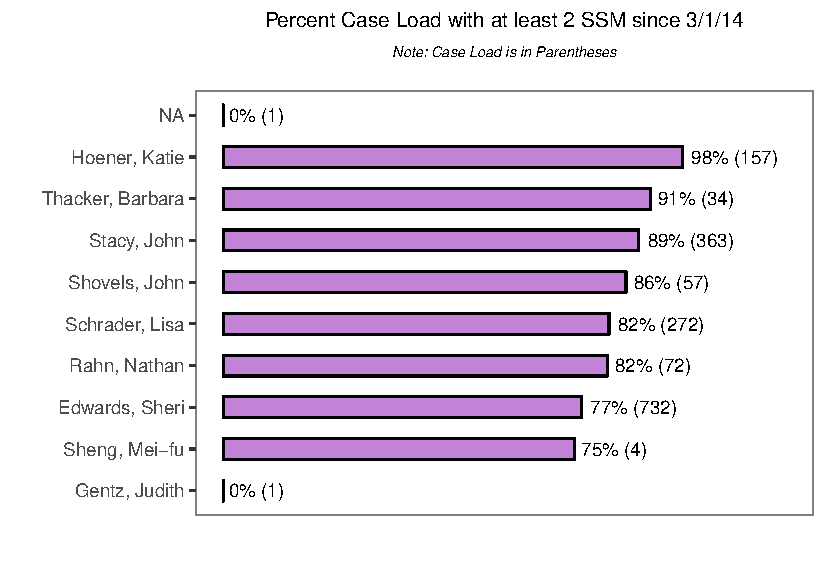
\includegraphics[width=\maxwidth]{figure/ssm-1} 

\end{knitrout}

\end{document}
